\documentclass[1p]{elsarticle_modified}
%\bibliographystyle{elsarticle-num}

%\usepackage[colorlinks]{hyperref}
%\usepackage{abbrmath_seonhwa} %\Abb, \Ascr, \Acal ,\Abf, \Afrak
\usepackage{amsfonts}
\usepackage{amssymb}
\usepackage{amsmath}
\usepackage{amsthm}
\usepackage{scalefnt}
\usepackage{amsbsy}
\usepackage{kotex}
\usepackage{caption}
\usepackage{subfig}
\usepackage{color}
\usepackage{graphicx}
\usepackage{xcolor} %% white, black, red, green, blue, cyan, magenta, yellow
\usepackage{float}
\usepackage{setspace}
\usepackage{hyperref}

\usepackage{tikz}
\usetikzlibrary{arrows}

\usepackage{multirow}
\usepackage{array} % fixed length table
\usepackage{hhline}

%%%%%%%%%%%%%%%%%%%%%
\makeatletter
\renewcommand*\env@matrix[1][\arraystretch]{%
	\edef\arraystretch{#1}%
	\hskip -\arraycolsep
	\let\@ifnextchar\new@ifnextchar
	\array{*\c@MaxMatrixCols c}}
\makeatother %https://tex.stackexchange.com/questions/14071/how-can-i-increase-the-line-spacing-in-a-matrix
%%%%%%%%%%%%%%%

\usepackage[normalem]{ulem}

\newcommand{\msout}[1]{\ifmmode\text{\sout{\ensuremath{#1}}}\else\sout{#1}\fi}
%SOURCE: \msout is \stkout macro in https://tex.stackexchange.com/questions/20609/strikeout-in-math-mode

\newcommand{\cancel}[1]{
	\ifmmode
	{\color{red}\msout{#1}}
	\else
	{\color{red}\sout{#1}}
	\fi
}

\newcommand{\add}[1]{
	{\color{blue}\uwave{#1}}
}

\newcommand{\replace}[2]{
	\ifmmode
	{\color{red}\msout{#1}}{\color{blue}\uwave{#2}}
	\else
	{\color{red}\sout{#1}}{\color{blue}\uwave{#2}}
	\fi
}

\newcommand{\Sol}{\mathcal{S}} %segment
\newcommand{\D}{D} %diagram
\newcommand{\A}{\mathcal{A}} %arc


%%%%%%%%%%%%%%%%%%%%%%%%%%%%%5 test

\def\sl{\operatorname{\textup{SL}}(2,\Cbb)}
\def\psl{\operatorname{\textup{PSL}}(2,\Cbb)}
\def\quan{\mkern 1mu \triangleright \mkern 1mu}

\theoremstyle{definition}
\newtheorem{thm}{Theorem}[section]
\newtheorem{prop}[thm]{Proposition}
\newtheorem{lem}[thm]{Lemma}
\newtheorem{ques}[thm]{Question}
\newtheorem{cor}[thm]{Corollary}
\newtheorem{defn}[thm]{Definition}
\newtheorem{exam}[thm]{Example}
\newtheorem{rmk}[thm]{Remark}
\newtheorem{alg}[thm]{Algorithm}

\newcommand{\I}{\sqrt{-1}}
\begin{document}

%\begin{frontmatter}
%
%\title{Boundary parabolic representations of knots up to 8 crossings}
%
%%% Group authors per affiliation:
%\author{Yunhi Cho} 
%\address{Department of Mathematics, University of Seoul, Seoul, Korea}
%\ead{yhcho@uos.ac.kr}
%
%
%\author{Seonhwa Kim} %\fnref{s_kim}}
%\address{Center for Geometry and Physics, Institute for Basic Science, Pohang, 37673, Korea}
%\ead{ryeona17@ibs.re.kr}
%
%\author{Hyuk Kim}
%\address{Department of Mathematical Sciences, Seoul National University, Seoul 08826, Korea}
%\ead{hyukkim@snu.ac.kr}
%
%\author{Seokbeom Yoon}
%\address{Department of Mathematical Sciences, Seoul National University, Seoul, 08826,  Korea}
%\ead{sbyoon15@snu.ac.kr}
%
%\begin{abstract}
%We find all boundary parabolic representation of knots up to 8 crossings.
%
%\end{abstract}
%\begin{keyword}
%    \MSC[2010] 57M25 
%\end{keyword}
%
%\end{frontmatter}

%\linenumbers
%\tableofcontents
%
\newcommand\colored[1]{\textcolor{white}{\rule[-0.35ex]{0.8em}{1.4ex}}\kern-0.8em\color{red} #1}%
%\newcommand\colored[1]{\textcolor{white}{ #1}\kern-2.17ex	\textcolor{white}{ #1}\kern-1.81ex	\textcolor{white}{ #1}\kern-2.15ex\color{red}#1	}

{\Large $\underline{12a_{0220}~(K12a_{0220})}$}

\setlength{\tabcolsep}{10pt}
\renewcommand{\arraystretch}{1.6}
\vspace{1cm}\begin{tabular}{m{100pt}>{\centering\arraybackslash}m{274pt}}
\multirow{5}{120pt}{
	\centering
	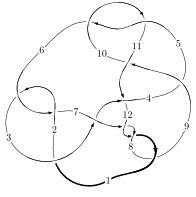
\includegraphics[width=112pt]{../../../GIT/diagram.site/Diagrams/png/1021_12a_0220.png}\\
\ \ \ A knot diagram\footnotemark}&
\allowdisplaybreaks
\textbf{Linearized knot diagam} \\
\cline{2-2}
 &
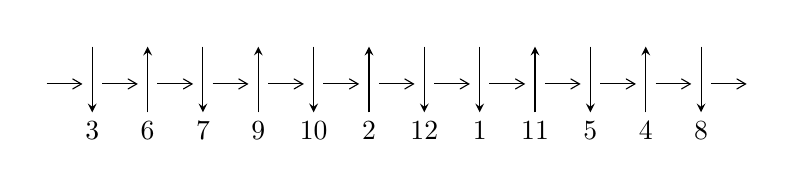
\begin{tikzpicture}[x=20pt, y=17pt]
	% nodes
	\node (C0) at (0, 0) {};
	\node (C1) at (1, 0) {};
	\node (C1U) at (1, +1) {};
	\node (C1D) at (1, -1) {3};

	\node (C2) at (2, 0) {};
	\node (C2U) at (2, +1) {};
	\node (C2D) at (2, -1) {6};

	\node (C3) at (3, 0) {};
	\node (C3U) at (3, +1) {};
	\node (C3D) at (3, -1) {7};

	\node (C4) at (4, 0) {};
	\node (C4U) at (4, +1) {};
	\node (C4D) at (4, -1) {9};

	\node (C5) at (5, 0) {};
	\node (C5U) at (5, +1) {};
	\node (C5D) at (5, -1) {10};

	\node (C6) at (6, 0) {};
	\node (C6U) at (6, +1) {};
	\node (C6D) at (6, -1) {2};

	\node (C7) at (7, 0) {};
	\node (C7U) at (7, +1) {};
	\node (C7D) at (7, -1) {12};

	\node (C8) at (8, 0) {};
	\node (C8U) at (8, +1) {};
	\node (C8D) at (8, -1) {1};

	\node (C9) at (9, 0) {};
	\node (C9U) at (9, +1) {};
	\node (C9D) at (9, -1) {11};

	\node (C10) at (10, 0) {};
	\node (C10U) at (10, +1) {};
	\node (C10D) at (10, -1) {5};

	\node (C11) at (11, 0) {};
	\node (C11U) at (11, +1) {};
	\node (C11D) at (11, -1) {4};

	\node (C12) at (12, 0) {};
	\node (C12U) at (12, +1) {};
	\node (C12D) at (12, -1) {8};
	\node (C13) at (13, 0) {};

	% arrows
	\draw[->,>={angle 60}]
	(C0) edge (C1) (C1) edge (C2) (C2) edge (C3) (C3) edge (C4) (C4) edge (C5) (C5) edge (C6) (C6) edge (C7) (C7) edge (C8) (C8) edge (C9) (C9) edge (C10) (C10) edge (C11) (C11) edge (C12) (C12) edge (C13) ;	\draw[->,>=stealth]
	(C1U) edge (C1D) (C2D) edge (C2U) (C3U) edge (C3D) (C4D) edge (C4U) (C5U) edge (C5D) (C6D) edge (C6U) (C7U) edge (C7D) (C8U) edge (C8D) (C9D) edge (C9U) (C10U) edge (C10D) (C11D) edge (C11U) (C12U) edge (C12D) ;
	\end{tikzpicture} \\
\hhline{~~} \\& 
\textbf{Solving Sequence} \\ \cline{2-2} 
 &
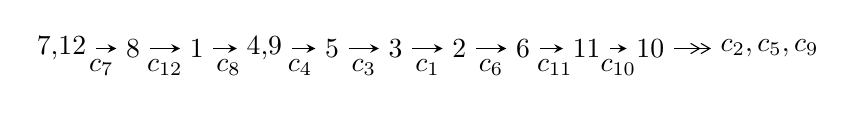
\begin{tikzpicture}[x=23pt, y=7pt]
	% node
	\node (A0) at (-1/8, 0) {7,12};
	\node (A1) at (1, 0) {8};
	\node (A2) at (2, 0) {1};
	\node (A3) at (49/16, 0) {4,9};
	\node (A4) at (33/8, 0) {5};
	\node (A5) at (41/8, 0) {3};
	\node (A6) at (49/8, 0) {2};
	\node (A7) at (57/8, 0) {6};
	\node (A8) at (65/8, 0) {11};
	\node (A9) at (73/8, 0) {10};
	\node (C1) at (1/2, -1) {$c_{7}$};
	\node (C2) at (3/2, -1) {$c_{12}$};
	\node (C3) at (5/2, -1) {$c_{8}$};
	\node (C4) at (29/8, -1) {$c_{4}$};
	\node (C5) at (37/8, -1) {$c_{3}$};
	\node (C6) at (45/8, -1) {$c_{1}$};
	\node (C7) at (53/8, -1) {$c_{6}$};
	\node (C8) at (61/8, -1) {$c_{11}$};
	\node (C9) at (69/8, -1) {$c_{10}$};
	\node (A10) at (11, 0) {$c_{2},c_{5},c_{9}$};

	% edge
	\draw[->,>=stealth]	
	(A0) edge (A1) (A1) edge (A2) (A2) edge (A3) (A3) edge (A4) (A4) edge (A5) (A5) edge (A6) (A6) edge (A7) (A7) edge (A8) (A8) edge (A9) ;
	\draw[->>,>={angle 60}]	
	(A9) edge (A10);
\end{tikzpicture} \\ 

\end{tabular} \\

\footnotetext{
The image of knot diagram is generated by the software ``\textbf{Draw programme}" developed by Andrew Bartholomew(\url{http://www.layer8.co.uk/maths/draw/index.htm\#Running-draw}), where we modified some parts for our purpose(\url{https://github.com/CATsTAILs/LinksPainter}).
}\phantom \\ \newline 
\centering \textbf{Ideals for irreducible components\footnotemark of $X_{\text{par}}$} 
 
\begin{align*}
I^u_{1}&=\langle 
-1.49096\times10^{181} u^{106}+9.13411\times10^{180} u^{105}+\cdots+5.06627\times10^{181} b-7.23078\times10^{182},\\
\phantom{I^u_{1}}&\phantom{= \langle  }6.06637\times10^{182} u^{106}-1.74049\times10^{183} u^{105}+\cdots+1.31723\times10^{183} a-2.71243\times10^{184},\\
\phantom{I^u_{1}}&\phantom{= \langle  }u^{107}-3 u^{106}+\cdots-111 u-13\rangle \\
I^u_{2}&=\langle 
b^2- b+1,\;a^4-2 a^2+2,\;u+1\rangle \\
I^u_{3}&=\langle 
b^2+b+1,\;a^3,\;u-1\rangle \\
\\
\end{align*}
\raggedright * 3 irreducible components of $\dim_{\mathbb{C}}=0$, with total 121 representations.\\
\footnotetext{All coefficients of polynomials are rational numbers. But the coefficients are sometimes approximated in decimal forms when there is not enough margin.}
\newpage
\renewcommand{\arraystretch}{1}
\centering \section*{I. $I^u_{1}= \langle -1.49\times10^{181} u^{106}+9.13\times10^{180} u^{105}+\cdots+5.07\times10^{181} b-7.23\times10^{182},\;6.07\times10^{182} u^{106}-1.74\times10^{183} u^{105}+\cdots+1.32\times10^{183} a-2.71\times10^{184},\;u^{107}-3 u^{106}+\cdots-111 u-13 \rangle$}
\flushleft \textbf{(i) Arc colorings}\\
\begin{tabular}{m{7pt} m{180pt} m{7pt} m{180pt} }
\flushright $a_{7}=$&$\begin{pmatrix}1\\0\end{pmatrix}$ \\
\flushright $a_{12}=$&$\begin{pmatrix}0\\u\end{pmatrix}$ \\
\flushright $a_{8}=$&$\begin{pmatrix}1\\u^2\end{pmatrix}$ \\
\flushright $a_{1}=$&$\begin{pmatrix}- u\\- u^3+u\end{pmatrix}$ \\
\flushright $a_{4}=$&$\begin{pmatrix}-0.460540 u^{106}+1.32132 u^{105}+\cdots+177.538 u+20.5919\\0.294291 u^{106}-0.180293 u^{105}+\cdots+132.884 u+14.2724\end{pmatrix}$ \\
\flushright $a_{9}=$&$\begin{pmatrix}- u^2+1\\- u^4+2 u^2\end{pmatrix}$ \\
\flushright $a_{5}=$&$\begin{pmatrix}-0.339961 u^{106}+1.59337 u^{105}+\cdots+324.599 u+34.4376\\0.183891 u^{106}-0.141636 u^{105}+\cdots+110.762 u+12.7655\end{pmatrix}$ \\
\flushright $a_{3}=$&$\begin{pmatrix}-0.166249 u^{106}+1.14103 u^{105}+\cdots+310.421 u+34.8643\\0.294291 u^{106}-0.180293 u^{105}+\cdots+132.884 u+14.2724\end{pmatrix}$ \\
\flushright $a_{2}=$&$\begin{pmatrix}-0.813218 u^{106}+2.47693 u^{105}+\cdots+392.711 u+41.8323\\-0.137167 u^{106}+0.176247 u^{105}+\cdots-14.8599 u-0.292318\end{pmatrix}$ \\
\flushright $a_{6}=$&$\begin{pmatrix}0.455592 u^{106}-2.01489 u^{105}+\cdots+4.63244 u+13.1807\\0.102062 u^{106}+0.00933752 u^{105}+\cdots-49.6066 u-10.5866\end{pmatrix}$ \\
\flushright $a_{11}=$&$\begin{pmatrix}-0.832717 u^{106}+1.95875 u^{105}+\cdots+267.318 u+30.0119\\-0.325817 u^{106}+0.776598 u^{105}+\cdots+23.5117 u+1.24472\end{pmatrix}$ \\
\flushright $a_{10}=$&$\begin{pmatrix}-0.816162 u^{106}+2.12713 u^{105}+\cdots+317.788 u+27.2416\\0.127653 u^{106}-0.129996 u^{105}+\cdots-43.6773 u-7.17967\end{pmatrix}$\\&\end{tabular}
\flushleft \textbf{(ii) Obstruction class $= -1$}\\~\\
\flushleft \textbf{(iii) Cusp Shapes $= -0.703236 u^{106}+1.11367 u^{105}+\cdots+8.19553 u+10.4291$}\\~\\
\newpage\renewcommand{\arraystretch}{1}
\flushleft \textbf{(iv) u-Polynomials at the component}\newline \\
\begin{tabular}{m{50pt}|m{274pt}}
Crossings & \hspace{64pt}u-Polynomials at each crossing \\
\hline $$\begin{aligned}c_{1}\end{aligned}$$&$\begin{aligned}
&u^{107}+54 u^{106}+\cdots-8 u-1
\end{aligned}$\\
\hline $$\begin{aligned}c_{2},c_{6}\end{aligned}$$&$\begin{aligned}
&u^{107}-2 u^{106}+\cdots+2 u-1
\end{aligned}$\\
\hline $$\begin{aligned}c_{3}\end{aligned}$$&$\begin{aligned}
&u^{107}+2 u^{106}+\cdots-188610 u-36209
\end{aligned}$\\
\hline $$\begin{aligned}c_{4}\end{aligned}$$&$\begin{aligned}
&u^{107}+u^{106}+\cdots+3876 u+3764
\end{aligned}$\\
\hline $$\begin{aligned}c_{5},c_{10}\end{aligned}$$&$\begin{aligned}
&u^{107}- u^{106}+\cdots+4 u+4
\end{aligned}$\\
\hline $$\begin{aligned}c_{7},c_{8},c_{12}\end{aligned}$$&$\begin{aligned}
&u^{107}+3 u^{106}+\cdots-111 u+13
\end{aligned}$\\
\hline $$\begin{aligned}c_{9}\end{aligned}$$&$\begin{aligned}
&u^{107}-51 u^{106}+\cdots-80 u+16
\end{aligned}$\\
\hline $$\begin{aligned}c_{11}\end{aligned}$$&$\begin{aligned}
&u^{107}-5 u^{106}+\cdots-692004 u+563884
\end{aligned}$\\
\hline
\end{tabular}\\~\\
\newpage\renewcommand{\arraystretch}{1}
\flushleft \textbf{(v) Riley Polynomials at the component}\newline \\
\begin{tabular}{m{50pt}|m{274pt}}
Crossings & \hspace{64pt}Riley Polynomials at each crossing \\
\hline $$\begin{aligned}c_{1}\end{aligned}$$&$\begin{aligned}
&y^{107}+6 y^{106}+\cdots+40 y-1
\end{aligned}$\\
\hline $$\begin{aligned}c_{2},c_{6}\end{aligned}$$&$\begin{aligned}
&y^{107}+54 y^{106}+\cdots-8 y-1
\end{aligned}$\\
\hline $$\begin{aligned}c_{3}\end{aligned}$$&$\begin{aligned}
&y^{107}-42 y^{106}+\cdots+2264493656 y-1311091681
\end{aligned}$\\
\hline $$\begin{aligned}c_{4}\end{aligned}$$&$\begin{aligned}
&y^{107}-21 y^{106}+\cdots+424757360 y-14167696
\end{aligned}$\\
\hline $$\begin{aligned}c_{5},c_{10}\end{aligned}$$&$\begin{aligned}
&y^{107}+51 y^{106}+\cdots-80 y-16
\end{aligned}$\\
\hline $$\begin{aligned}c_{7},c_{8},c_{12}\end{aligned}$$&$\begin{aligned}
&y^{107}-103 y^{106}+\cdots-9207 y-169
\end{aligned}$\\
\hline $$\begin{aligned}c_{9}\end{aligned}$$&$\begin{aligned}
&y^{107}+15 y^{106}+\cdots-2304 y-256
\end{aligned}$\\
\hline $$\begin{aligned}c_{11}\end{aligned}$$&$\begin{aligned}
&y^{107}+39 y^{106}+\cdots-10755598905296 y-317965165456
\end{aligned}$\\
\hline
\end{tabular}\\~\\
\newpage\flushleft \textbf{(vi) Complex Volumes and Cusp Shapes}
$$\begin{array}{c|c|c}  
\text{Solutions to }I^u_{1}& \I (\text{vol} + \sqrt{-1}CS) & \text{Cusp shape}\\
 \hline 
\begin{aligned}
u &= -0.904262 + 0.431584 I \\
a &= -0.133296 - 0.339278 I \\
b &= \phantom{-}0.530938 - 0.189035 I\end{aligned}
 & -1.99885 + 5.17052 I & \phantom{-0.000000 } 0 \\ \hline\begin{aligned}
u &= -0.904262 - 0.431584 I \\
a &= -0.133296 + 0.339278 I \\
b &= \phantom{-}0.530938 + 0.189035 I\end{aligned}
 & -1.99885 - 5.17052 I & \phantom{-0.000000 } 0 \\ \hline\begin{aligned}
u &= \phantom{-}0.787760 + 0.643206 I \\
a &= \phantom{-}0.871626 + 0.708841 I \\
b &= -1.096750 + 0.335060 I\end{aligned}
 & -4.40852 + 2.42869 I & \phantom{-0.000000 } 0 \\ \hline\begin{aligned}
u &= \phantom{-}0.787760 - 0.643206 I \\
a &= \phantom{-}0.871626 - 0.708841 I \\
b &= -1.096750 - 0.335060 I\end{aligned}
 & -4.40852 - 2.42869 I & \phantom{-0.000000 } 0 \\ \hline\begin{aligned}
u &= -0.956946 + 0.360565 I \\
a &= -0.597535 + 0.227282 I \\
b &= \phantom{-}0.958606 + 0.767416 I\end{aligned}
 & -0.373093 - 0.971380 I & \phantom{-0.000000 } 0 \\ \hline\begin{aligned}
u &= -0.956946 - 0.360565 I \\
a &= -0.597535 - 0.227282 I \\
b &= \phantom{-}0.958606 - 0.767416 I\end{aligned}
 & -0.373093 + 0.971380 I & \phantom{-0.000000 } 0 \\ \hline\begin{aligned}
u &= -0.358282 + 0.896448 I \\
a &= -1.10747 + 1.21913 I \\
b &= \phantom{-}1.41980 - 0.65124 I\end{aligned}
 & -1.00079 + 12.66400 I & \phantom{-0.000000 } 0 \\ \hline\begin{aligned}
u &= -0.358282 - 0.896448 I \\
a &= -1.10747 - 1.21913 I \\
b &= \phantom{-}1.41980 + 0.65124 I\end{aligned}
 & -1.00079 - 12.66400 I & \phantom{-0.000000 } 0 \\ \hline\begin{aligned}
u &= \phantom{-}0.992483 + 0.309368 I \\
a &= -0.160962 - 0.486626 I \\
b &= -0.269567 - 0.291149 I\end{aligned}
 & -3.00656 - 1.10116 I & \phantom{-0.000000 } 0 \\ \hline\begin{aligned}
u &= \phantom{-}0.992483 - 0.309368 I \\
a &= -0.160962 + 0.486626 I \\
b &= -0.269567 + 0.291149 I\end{aligned}
 & -3.00656 + 1.10116 I & \phantom{-0.000000 } 0\\
 \hline 
 \end{array}$$\newpage$$\begin{array}{c|c|c}  
\text{Solutions to }I^u_{1}& \I (\text{vol} + \sqrt{-1}CS) & \text{Cusp shape}\\
 \hline 
\begin{aligned}
u &= -0.608114 + 0.728544 I \\
a &= -0.691648 + 0.449361 I \\
b &= \phantom{-}1.128540 - 0.315477 I\end{aligned}
 & -2.81110 + 0.44680 I & \phantom{-0.000000 } 0 \\ \hline\begin{aligned}
u &= -0.608114 - 0.728544 I \\
a &= -0.691648 - 0.449361 I \\
b &= \phantom{-}1.128540 + 0.315477 I\end{aligned}
 & -2.81110 - 0.44680 I & \phantom{-0.000000 } 0 \\ \hline\begin{aligned}
u &= \phantom{-}1.033090 + 0.207124 I \\
a &= -0.748487 - 0.391269 I \\
b &= \phantom{-}0.001488 - 0.410585 I\end{aligned}
 & -1.89971 - 0.44446 I & \phantom{-0.000000 } 0 \\ \hline\begin{aligned}
u &= \phantom{-}1.033090 - 0.207124 I \\
a &= -0.748487 + 0.391269 I \\
b &= \phantom{-}0.001488 + 0.410585 I\end{aligned}
 & -1.89971 + 0.44446 I & \phantom{-0.000000 } 0 \\ \hline\begin{aligned}
u &= \phantom{-}0.391004 + 0.857866 I \\
a &= \phantom{-}0.99548 + 1.11660 I \\
b &= -1.36178 - 0.60152 I\end{aligned}
 & -3.15539 - 7.60366 I & \phantom{-0.000000 } 0 \\ \hline\begin{aligned}
u &= \phantom{-}0.391004 - 0.857866 I \\
a &= \phantom{-}0.99548 - 1.11660 I \\
b &= -1.36178 + 0.60152 I\end{aligned}
 & -3.15539 + 7.60366 I & \phantom{-0.000000 } 0 \\ \hline\begin{aligned}
u &= -0.541436 + 0.770509 I \\
a &= -0.741344 + 1.076260 I \\
b &= \phantom{-}0.858958 - 0.011904 I\end{aligned}
 & -2.59503 + 4.68959 I & \phantom{-0.000000 } 0 \\ \hline\begin{aligned}
u &= -0.541436 - 0.770509 I \\
a &= -0.741344 - 1.076260 I \\
b &= \phantom{-}0.858958 + 0.011904 I\end{aligned}
 & -2.59503 - 4.68959 I & \phantom{-0.000000 } 0 \\ \hline\begin{aligned}
u &= \phantom{-}0.606025 + 0.712743 I \\
a &= \phantom{-}0.766219 + 0.966722 I \\
b &= -0.916895 + 0.108302 I\end{aligned}
 & -4.40673 + 0.22528 I & \phantom{-0.000000 } 0 \\ \hline\begin{aligned}
u &= \phantom{-}0.606025 - 0.712743 I \\
a &= \phantom{-}0.766219 - 0.966722 I \\
b &= -0.916895 - 0.108302 I\end{aligned}
 & -4.40673 - 0.22528 I & \phantom{-0.000000 } 0\\
 \hline 
 \end{array}$$\newpage$$\begin{array}{c|c|c}  
\text{Solutions to }I^u_{1}& \I (\text{vol} + \sqrt{-1}CS) & \text{Cusp shape}\\
 \hline 
\begin{aligned}
u &= -1.023130 + 0.308756 I \\
a &= \phantom{-}0.835122 + 0.060413 I \\
b &= -0.362952 - 0.673846 I\end{aligned}
 & \phantom{-}1.30429 + 3.26731 I & \phantom{-0.000000 } 0 \\ \hline\begin{aligned}
u &= -1.023130 - 0.308756 I \\
a &= \phantom{-}0.835122 - 0.060413 I \\
b &= -0.362952 + 0.673846 I\end{aligned}
 & \phantom{-}1.30429 - 3.26731 I & \phantom{-0.000000 } 0 \\ \hline\begin{aligned}
u &= \phantom{-}0.517016 + 0.772169 I \\
a &= \phantom{-}0.775725 + 0.721111 I \\
b &= -1.220000 - 0.429494 I\end{aligned}
 & -4.10761 - 5.28481 I & \phantom{-0.000000 } 0 \\ \hline\begin{aligned}
u &= \phantom{-}0.517016 - 0.772169 I \\
a &= \phantom{-}0.775725 - 0.721111 I \\
b &= -1.220000 + 0.429494 I\end{aligned}
 & -4.10761 + 5.28481 I & \phantom{-0.000000 } 0 \\ \hline\begin{aligned}
u &= -0.873419 + 0.646269 I \\
a &= -0.961755 + 0.599798 I \\
b &= \phantom{-}1.201530 + 0.414908 I\end{aligned}
 & -2.58534 - 7.32575 I & \phantom{-0.000000 } 0 \\ \hline\begin{aligned}
u &= -0.873419 - 0.646269 I \\
a &= -0.961755 - 0.599798 I \\
b &= \phantom{-}1.201530 - 0.414908 I\end{aligned}
 & -2.58534 + 7.32575 I & \phantom{-0.000000 } 0 \\ \hline\begin{aligned}
u &= -1.073390 + 0.173489 I \\
a &= \phantom{-}1.185970 - 0.495544 I \\
b &= \phantom{-}0.025415 - 0.404365 I\end{aligned}
 & \phantom{-}0.62750 - 3.83015 I & \phantom{-0.000000 } 0 \\ \hline\begin{aligned}
u &= -1.073390 - 0.173489 I \\
a &= \phantom{-}1.185970 + 0.495544 I \\
b &= \phantom{-}0.025415 + 0.404365 I\end{aligned}
 & \phantom{-}0.62750 + 3.83015 I & \phantom{-0.000000 } 0 \\ \hline\begin{aligned}
u &= -0.347205 + 0.789149 I \\
a &= \phantom{-}0.98779 - 1.36315 I \\
b &= -0.998853 + 0.689661 I\end{aligned}
 & \phantom{-}1.55865 + 7.81274 I & \phantom{-0.000000 } 0 \\ \hline\begin{aligned}
u &= -0.347205 - 0.789149 I \\
a &= \phantom{-}0.98779 + 1.36315 I \\
b &= -0.998853 - 0.689661 I\end{aligned}
 & \phantom{-}1.55865 - 7.81274 I & \phantom{-0.000000 } 0\\
 \hline 
 \end{array}$$\newpage$$\begin{array}{c|c|c}  
\text{Solutions to }I^u_{1}& \I (\text{vol} + \sqrt{-1}CS) & \text{Cusp shape}\\
 \hline 
\begin{aligned}
u &= -0.697681 + 0.486866 I \\
a &= \phantom{-}1.017260 - 0.382052 I \\
b &= -0.787593 - 0.084239 I\end{aligned}
 & \phantom{-}0.26585 - 3.31149 I & \phantom{-0.000000 } 0 \\ \hline\begin{aligned}
u &= -0.697681 - 0.486866 I \\
a &= \phantom{-}1.017260 + 0.382052 I \\
b &= -0.787593 + 0.084239 I\end{aligned}
 & \phantom{-}0.26585 + 3.31149 I & \phantom{-0.000000 } 0 \\ \hline\begin{aligned}
u &= -0.305416 + 0.776614 I \\
a &= -0.73060 + 1.37269 I \\
b &= \phantom{-}1.24517 - 0.72111 I\end{aligned}
 & \phantom{-}1.49738 + 5.20503 I & \phantom{-0.000000 } 0 \\ \hline\begin{aligned}
u &= -0.305416 - 0.776614 I \\
a &= -0.73060 - 1.37269 I \\
b &= \phantom{-}1.24517 + 0.72111 I\end{aligned}
 & \phantom{-}1.49738 - 5.20503 I & \phantom{-0.000000 } 0 \\ \hline\begin{aligned}
u &= \phantom{-}0.366231 + 0.724436 I \\
a &= -0.89880 - 1.21010 I \\
b &= \phantom{-}0.918174 + 0.589822 I\end{aligned}
 & -0.58468 - 2.93122 I & \phantom{-0.000000 } 0 \\ \hline\begin{aligned}
u &= \phantom{-}0.366231 - 0.724436 I \\
a &= -0.89880 + 1.21010 I \\
b &= \phantom{-}0.918174 - 0.589822 I\end{aligned}
 & -0.58468 + 2.93122 I & \phantom{-0.000000 } 0 \\ \hline\begin{aligned}
u &= -1.193830 + 0.133951 I \\
a &= \phantom{-}1.186440 + 0.254501 I \\
b &= \phantom{-}0.478845 - 0.410517 I\end{aligned}
 & \phantom{-}1.09290 + 3.87383 I & \phantom{-0.000000 } 0 \\ \hline\begin{aligned}
u &= -1.193830 - 0.133951 I \\
a &= \phantom{-}1.186440 - 0.254501 I \\
b &= \phantom{-}0.478845 + 0.410517 I\end{aligned}
 & \phantom{-}1.09290 - 3.87383 I & \phantom{-0.000000 } 0 \\ \hline\begin{aligned}
u &= \phantom{-}1.201360 + 0.183444 I \\
a &= \phantom{-}0.419710 - 0.338240 I \\
b &= -0.79913 + 1.21442 I\end{aligned}
 & -0.18627 + 3.28365 I & \phantom{-0.000000 } 0 \\ \hline\begin{aligned}
u &= \phantom{-}1.201360 - 0.183444 I \\
a &= \phantom{-}0.419710 + 0.338240 I \\
b &= -0.79913 - 1.21442 I\end{aligned}
 & -0.18627 - 3.28365 I & \phantom{-0.000000 } 0\\
 \hline 
 \end{array}$$\newpage$$\begin{array}{c|c|c}  
\text{Solutions to }I^u_{1}& \I (\text{vol} + \sqrt{-1}CS) & \text{Cusp shape}\\
 \hline 
\begin{aligned}
u &= \phantom{-}1.24303\phantom{ +0.000000I} \\
a &= -0.920747\phantom{ +0.000000I} \\
b &= -0.643030\phantom{ +0.000000I}\end{aligned}
 & -2.16232\phantom{ +0.000000I} & \phantom{-0.000000 } 0 \\ \hline\begin{aligned}
u &= -0.222910 + 0.706813 I \\
a &= \phantom{-}0.57898 - 1.45300 I \\
b &= -0.731318 + 0.783769 I\end{aligned}
 & \phantom{-}3.66702 + 0.52581 I & \phantom{-}4.89543 - 0.81246 I \\ \hline\begin{aligned}
u &= -0.222910 - 0.706813 I \\
a &= \phantom{-}0.57898 + 1.45300 I \\
b &= -0.731318 - 0.783769 I\end{aligned}
 & \phantom{-}3.66702 - 0.52581 I & \phantom{-}4.89543 + 0.81246 I \\ \hline\begin{aligned}
u &= \phantom{-}0.504839 + 0.540212 I \\
a &= -0.851823 - 0.684157 I \\
b &= \phantom{-}0.771656 + 0.223252 I\end{aligned}
 & -1.33042 - 1.16536 I & -4.57238 + 3.59666 I \\ \hline\begin{aligned}
u &= \phantom{-}0.504839 - 0.540212 I \\
a &= -0.851823 + 0.684157 I \\
b &= \phantom{-}0.771656 - 0.223252 I\end{aligned}
 & -1.33042 + 1.16536 I & -4.57238 - 3.59666 I \\ \hline\begin{aligned}
u &= \phantom{-}1.245520 + 0.201441 I \\
a &= -0.458006 + 0.563615 I \\
b &= \phantom{-}0.050412 - 1.311980 I\end{aligned}
 & \phantom{-}0.58850 - 1.75903 I & \phantom{-0.000000 } 0 \\ \hline\begin{aligned}
u &= \phantom{-}1.245520 - 0.201441 I \\
a &= -0.458006 - 0.563615 I \\
b &= \phantom{-}0.050412 + 1.311980 I\end{aligned}
 & \phantom{-}0.58850 + 1.75903 I & \phantom{-0.000000 } 0 \\ \hline\begin{aligned}
u &= -1.346650 + 0.022218 I \\
a &= -0.127155 - 0.744802 I \\
b &= \phantom{-}0.49820 + 1.55717 I\end{aligned}
 & -3.79047 - 1.76476 I & \phantom{-0.000000 } 0 \\ \hline\begin{aligned}
u &= -1.346650 - 0.022218 I \\
a &= -0.127155 + 0.744802 I \\
b &= \phantom{-}0.49820 - 1.55717 I\end{aligned}
 & -3.79047 + 1.76476 I & \phantom{-0.000000 } 0 \\ \hline\begin{aligned}
u &= -1.349610 + 0.062394 I \\
a &= -1.345650 + 0.408342 I \\
b &= -1.030110 + 0.398339 I\end{aligned}
 & -1.64321 - 0.63614 I & \phantom{-0.000000 } 0\\
 \hline 
 \end{array}$$\newpage$$\begin{array}{c|c|c}  
\text{Solutions to }I^u_{1}& \I (\text{vol} + \sqrt{-1}CS) & \text{Cusp shape}\\
 \hline 
\begin{aligned}
u &= -1.349610 - 0.062394 I \\
a &= -1.345650 - 0.408342 I \\
b &= -1.030110 - 0.398339 I\end{aligned}
 & -1.64321 + 0.63614 I & \phantom{-0.000000 } 0 \\ \hline\begin{aligned}
u &= -1.356410 + 0.112287 I \\
a &= \phantom{-}0.202197 + 0.820758 I \\
b &= \phantom{-}0.17434 - 1.59862 I\end{aligned}
 & -3.53567 + 3.73820 I & \phantom{-0.000000 } 0 \\ \hline\begin{aligned}
u &= -1.356410 - 0.112287 I \\
a &= \phantom{-}0.202197 - 0.820758 I \\
b &= \phantom{-}0.17434 + 1.59862 I\end{aligned}
 & -3.53567 - 3.73820 I & \phantom{-0.000000 } 0 \\ \hline\begin{aligned}
u &= -1.358470 + 0.143026 I \\
a &= -1.353580 - 0.228884 I \\
b &= -1.160700 + 0.526570 I\end{aligned}
 & -1.26765 + 7.94095 I & \phantom{-0.000000 } 0 \\ \hline\begin{aligned}
u &= -1.358470 - 0.143026 I \\
a &= -1.353580 + 0.228884 I \\
b &= -1.160700 - 0.526570 I\end{aligned}
 & -1.26765 - 7.94095 I & \phantom{-0.000000 } 0 \\ \hline\begin{aligned}
u &= \phantom{-}1.368360 + 0.085834 I \\
a &= \phantom{-}0.290701 - 0.765642 I \\
b &= -0.64968 + 1.59002 I\end{aligned}
 & -2.02551 - 3.00487 I & \phantom{-0.000000 } 0 \\ \hline\begin{aligned}
u &= \phantom{-}1.368360 - 0.085834 I \\
a &= \phantom{-}0.290701 + 0.765642 I \\
b &= -0.64968 - 1.59002 I\end{aligned}
 & -2.02551 + 3.00487 I & \phantom{-0.000000 } 0 \\ \hline\begin{aligned}
u &= \phantom{-}1.379890 + 0.160353 I \\
a &= -0.317648 + 0.896210 I \\
b &= -0.05306 - 1.66215 I\end{aligned}
 & -1.56942 - 8.60645 I & \phantom{-0.000000 } 0 \\ \hline\begin{aligned}
u &= \phantom{-}1.379890 - 0.160353 I \\
a &= -0.317648 - 0.896210 I \\
b &= -0.05306 + 1.66215 I\end{aligned}
 & -1.56942 + 8.60645 I & \phantom{-0.000000 } 0 \\ \hline\begin{aligned}
u &= \phantom{-}1.390970 + 0.096096 I \\
a &= \phantom{-}1.103970 + 0.103885 I \\
b &= \phantom{-}1.152920 + 0.397138 I\end{aligned}
 & -4.97509 - 3.82300 I & \phantom{-0.000000 } 0\\
 \hline 
 \end{array}$$\newpage$$\begin{array}{c|c|c}  
\text{Solutions to }I^u_{1}& \I (\text{vol} + \sqrt{-1}CS) & \text{Cusp shape}\\
 \hline 
\begin{aligned}
u &= \phantom{-}1.390970 - 0.096096 I \\
a &= \phantom{-}1.103970 - 0.103885 I \\
b &= \phantom{-}1.152920 - 0.397138 I\end{aligned}
 & -4.97509 + 3.82300 I & \phantom{-0.000000 } 0 \\ \hline\begin{aligned}
u &= -0.037503 + 0.596397 I \\
a &= \phantom{-}0.36414 - 1.92620 I \\
b &= \phantom{-}0.261674 + 1.022480 I\end{aligned}
 & \phantom{-}4.52566 - 1.15109 I & \phantom{-}6.23436 + 0.38594 I \\ \hline\begin{aligned}
u &= -0.037503 - 0.596397 I \\
a &= \phantom{-}0.36414 + 1.92620 I \\
b &= \phantom{-}0.261674 - 1.022480 I\end{aligned}
 & \phantom{-}4.52566 + 1.15109 I & \phantom{-}6.23436 - 0.38594 I \\ \hline\begin{aligned}
u &= \phantom{-}1.40667 + 0.26184 I \\
a &= -0.485247 + 0.970070 I \\
b &= -1.141110 - 0.816619 I\end{aligned}
 & -1.56131 - 4.01030 I & \phantom{-0.000000 } 0 \\ \hline\begin{aligned}
u &= \phantom{-}1.40667 - 0.26184 I \\
a &= -0.485247 - 0.970070 I \\
b &= -1.141110 + 0.816619 I\end{aligned}
 & -1.56131 + 4.01030 I & \phantom{-0.000000 } 0 \\ \hline\begin{aligned}
u &= -0.298161 + 0.443295 I \\
a &= -0.549122 + 0.963108 I \\
b &= \phantom{-}0.444626 + 0.356044 I\end{aligned}
 & -0.15371 - 1.58994 I & -1.42624 + 1.98288 I \\ \hline\begin{aligned}
u &= -0.298161 - 0.443295 I \\
a &= -0.549122 - 0.963108 I \\
b &= \phantom{-}0.444626 - 0.356044 I\end{aligned}
 & -0.15371 + 1.58994 I & -1.42624 - 1.98288 I \\ \hline\begin{aligned}
u &= \phantom{-}1.46362 + 0.17385 I \\
a &= \phantom{-}0.304404 - 1.032320 I \\
b &= \phantom{-}0.846992 + 0.221001 I\end{aligned}
 & -6.17519 - 0.76182 I & \phantom{-0.000000 } 0 \\ \hline\begin{aligned}
u &= \phantom{-}1.46362 - 0.17385 I \\
a &= \phantom{-}0.304404 + 1.032320 I \\
b &= \phantom{-}0.846992 - 0.221001 I\end{aligned}
 & -6.17519 + 0.76182 I & \phantom{-0.000000 } 0 \\ \hline\begin{aligned}
u &= -0.155990 + 0.497529 I \\
a &= \phantom{-}1.04483 - 2.35071 I \\
b &= \phantom{-}0.015047 + 1.085040 I\end{aligned}
 & \phantom{-}3.36815 + 6.26844 I & \phantom{-}3.96391 - 7.68382 I\\
 \hline 
 \end{array}$$\newpage$$\begin{array}{c|c|c}  
\text{Solutions to }I^u_{1}& \I (\text{vol} + \sqrt{-1}CS) & \text{Cusp shape}\\
 \hline 
\begin{aligned}
u &= -0.155990 - 0.497529 I \\
a &= \phantom{-}1.04483 + 2.35071 I \\
b &= \phantom{-}0.015047 - 1.085040 I\end{aligned}
 & \phantom{-}3.36815 - 6.26844 I & \phantom{-}3.96391 + 7.68382 I \\ \hline\begin{aligned}
u &= \phantom{-}1.44935 + 0.30104 I \\
a &= \phantom{-}0.526429 - 1.065710 I \\
b &= \phantom{-}1.52911 + 0.71038 I\end{aligned}
 & -4.15695 - 9.12120 I & \phantom{-0.000000 } 0 \\ \hline\begin{aligned}
u &= \phantom{-}1.44935 - 0.30104 I \\
a &= \phantom{-}0.526429 + 1.065710 I \\
b &= \phantom{-}1.52911 - 0.71038 I\end{aligned}
 & -4.15695 + 9.12120 I & \phantom{-0.000000 } 0 \\ \hline\begin{aligned}
u &= -1.46542 + 0.27690 I \\
a &= \phantom{-}0.254920 + 1.037850 I \\
b &= \phantom{-}1.32007 - 0.86889 I\end{aligned}
 & -6.50073 + 6.60004 I & \phantom{-0.000000 } 0 \\ \hline\begin{aligned}
u &= -1.46542 - 0.27690 I \\
a &= \phantom{-}0.254920 - 1.037850 I \\
b &= \phantom{-}1.32007 + 0.86889 I\end{aligned}
 & -6.50073 - 6.60004 I & \phantom{-0.000000 } 0 \\ \hline\begin{aligned}
u &= \phantom{-}1.46386 + 0.30484 I \\
a &= -0.263373 + 1.147230 I \\
b &= -1.31153 - 0.95461 I\end{aligned}
 & -4.27302 - 11.79580 I & \phantom{-0.000000 } 0 \\ \hline\begin{aligned}
u &= \phantom{-}1.46386 - 0.30484 I \\
a &= -0.263373 - 1.147230 I \\
b &= -1.31153 + 0.95461 I\end{aligned}
 & -4.27302 + 11.79580 I & \phantom{-0.000000 } 0 \\ \hline\begin{aligned}
u &= -1.48495 + 0.19479 I \\
a &= \phantom{-}0.167816 + 0.722945 I \\
b &= \phantom{-}1.38966 - 0.61548 I\end{aligned}
 & -7.76705 + 3.90228 I & \phantom{-0.000000 } 0 \\ \hline\begin{aligned}
u &= -1.48495 - 0.19479 I \\
a &= \phantom{-}0.167816 - 0.722945 I \\
b &= \phantom{-}1.38966 + 0.61548 I\end{aligned}
 & -7.76705 - 3.90228 I & \phantom{-0.000000 } 0 \\ \hline\begin{aligned}
u &= \phantom{-}1.49176 + 0.14550 I \\
a &= -0.134205 + 0.537263 I \\
b &= -1.41496 - 0.46095 I\end{aligned}
 & -6.68330 + 1.19848 I & \phantom{-0.000000 } 0\\
 \hline 
 \end{array}$$\newpage$$\begin{array}{c|c|c}  
\text{Solutions to }I^u_{1}& \I (\text{vol} + \sqrt{-1}CS) & \text{Cusp shape}\\
 \hline 
\begin{aligned}
u &= \phantom{-}1.49176 - 0.14550 I \\
a &= -0.134205 - 0.537263 I \\
b &= -1.41496 + 0.46095 I\end{aligned}
 & -6.68330 - 1.19848 I & \phantom{-0.000000 } 0 \\ \hline\begin{aligned}
u &= \phantom{-}0.066760 + 0.486078 I \\
a &= -0.41695 + 2.46615 I \\
b &= -0.881052 - 0.937770 I\end{aligned}
 & \phantom{-}3.30433 - 5.76662 I & \phantom{-}3.79923 + 6.91273 I \\ \hline\begin{aligned}
u &= \phantom{-}0.066760 - 0.486078 I \\
a &= -0.41695 - 2.46615 I \\
b &= -0.881052 + 0.937770 I\end{aligned}
 & \phantom{-}3.30433 + 5.76662 I & \phantom{-}3.79923 - 6.91273 I \\ \hline\begin{aligned}
u &= \phantom{-}1.48454 + 0.34898 I \\
a &= \phantom{-}0.254201 - 1.213360 I \\
b &= \phantom{-}1.65526 + 0.76856 I\end{aligned}
 & -6.9227 - 17.1759 I & \phantom{-0.000000 } 0 \\ \hline\begin{aligned}
u &= \phantom{-}1.48454 - 0.34898 I \\
a &= \phantom{-}0.254201 + 1.213360 I \\
b &= \phantom{-}1.65526 - 0.76856 I\end{aligned}
 & -6.9227 + 17.1759 I & \phantom{-0.000000 } 0 \\ \hline\begin{aligned}
u &= -1.49146 + 0.32588 I \\
a &= -0.272333 - 1.094210 I \\
b &= -1.64360 + 0.71264 I\end{aligned}
 & -9.2253 + 11.9036 I & \phantom{-0.000000 } 0 \\ \hline\begin{aligned}
u &= -1.49146 - 0.32588 I \\
a &= -0.272333 + 1.094210 I \\
b &= -1.64360 - 0.71264 I\end{aligned}
 & -9.2253 - 11.9036 I & \phantom{-0.000000 } 0 \\ \hline\begin{aligned}
u &= \phantom{-}0.066503 + 0.460813 I \\
a &= -1.13702 - 1.73349 I \\
b &= -0.034938 + 0.934134 I\end{aligned}
 & \phantom{-}0.95866 - 1.83427 I & \phantom{-}0.73406 + 3.89858 I \\ \hline\begin{aligned}
u &= \phantom{-}0.066503 - 0.460813 I \\
a &= -1.13702 + 1.73349 I \\
b &= -0.034938 - 0.934134 I\end{aligned}
 & \phantom{-}0.95866 + 1.83427 I & \phantom{-}0.73406 - 3.89858 I \\ \hline\begin{aligned}
u &= -1.52227 + 0.25706 I \\
a &= -0.251276 - 0.717849 I \\
b &= -1.62467 + 0.53247 I\end{aligned}
 & -10.77400 + 9.01109 I & \phantom{-0.000000 } 0\\
 \hline 
 \end{array}$$\newpage$$\begin{array}{c|c|c}  
\text{Solutions to }I^u_{1}& \I (\text{vol} + \sqrt{-1}CS) & \text{Cusp shape}\\
 \hline 
\begin{aligned}
u &= -1.52227 - 0.25706 I \\
a &= -0.251276 + 0.717849 I \\
b &= -1.62467 - 0.53247 I\end{aligned}
 & -10.77400 - 9.01109 I & \phantom{-0.000000 } 0 \\ \hline\begin{aligned}
u &= \phantom{-}1.53098 + 0.21479 I \\
a &= \phantom{-}0.265871 - 0.505711 I \\
b &= \phantom{-}1.58794 + 0.43363 I\end{aligned}
 & -9.84860 - 3.77356 I & \phantom{-0.000000 } 0 \\ \hline\begin{aligned}
u &= \phantom{-}1.53098 - 0.21479 I \\
a &= \phantom{-}0.265871 + 0.505711 I \\
b &= \phantom{-}1.58794 - 0.43363 I\end{aligned}
 & -9.84860 + 3.77356 I & \phantom{-0.000000 } 0 \\ \hline\begin{aligned}
u &= \phantom{-}1.52612 + 0.24737 I \\
a &= \phantom{-}0.153500 - 1.100690 I \\
b &= \phantom{-}0.833157 + 0.473629 I\end{aligned}
 & -9.36969 - 8.34998 I & \phantom{-0.000000 } 0 \\ \hline\begin{aligned}
u &= \phantom{-}1.52612 - 0.24737 I \\
a &= \phantom{-}0.153500 + 1.100690 I \\
b &= \phantom{-}0.833157 - 0.473629 I\end{aligned}
 & -9.36969 + 8.34998 I & \phantom{-0.000000 } 0 \\ \hline\begin{aligned}
u &= -1.53189 + 0.21291 I \\
a &= -0.156064 - 1.042910 I \\
b &= -0.907267 + 0.417953 I\end{aligned}
 & -11.43450 + 3.06093 I & \phantom{-0.000000 } 0 \\ \hline\begin{aligned}
u &= -1.53189 - 0.21291 I \\
a &= -0.156064 + 1.042910 I \\
b &= -0.907267 - 0.417953 I\end{aligned}
 & -11.43450 - 3.06093 I & \phantom{-0.000000 } 0 \\ \hline\begin{aligned}
u &= -1.55684 + 0.12305 I \\
a &= -0.148490 - 0.836226 I \\
b &= -1.116250 + 0.286900 I\end{aligned}
 & -12.31450 + 0.01828 I & \phantom{-0.000000 } 0 \\ \hline\begin{aligned}
u &= -1.55684 - 0.12305 I \\
a &= -0.148490 + 0.836226 I \\
b &= -1.116250 - 0.286900 I\end{aligned}
 & -12.31450 - 0.01828 I & \phantom{-0.000000 } 0 \\ \hline\begin{aligned}
u &= \phantom{-}1.56528 + 0.07740 I \\
a &= \phantom{-}0.149063 - 0.704571 I \\
b &= \phantom{-}1.211780 + 0.210713 I\end{aligned}
 & -11.02690 + 5.25826 I & \phantom{-0.000000 } 0\\
 \hline 
 \end{array}$$\newpage$$\begin{array}{c|c|c}  
\text{Solutions to }I^u_{1}& \I (\text{vol} + \sqrt{-1}CS) & \text{Cusp shape}\\
 \hline 
\begin{aligned}
u &= \phantom{-}1.56528 - 0.07740 I \\
a &= \phantom{-}0.149063 + 0.704571 I \\
b &= \phantom{-}1.211780 - 0.210713 I\end{aligned}
 & -11.02690 - 5.25826 I & \phantom{-0.000000 } 0 \\ \hline\begin{aligned}
u &= -0.154957 + 0.386807 I \\
a &= -0.836798 + 0.702949 I \\
b &= \phantom{-}0.264901 + 0.471924 I\end{aligned}
 & -0.14462 - 1.60637 I & -1.48281 + 3.72848 I \\ \hline\begin{aligned}
u &= -0.154957 - 0.386807 I \\
a &= -0.836798 - 0.702949 I \\
b &= \phantom{-}0.264901 - 0.471924 I\end{aligned}
 & -0.14462 + 1.60637 I & -1.48281 - 3.72848 I \\ \hline\begin{aligned}
u &= -0.156750 + 0.282652 I \\
a &= \phantom{-}2.02349 + 1.65973 I \\
b &= \phantom{-}0.732640 - 0.821272 I\end{aligned}
 & \phantom{-}0.05214 + 2.40475 I & -0.47032 - 3.52067 I \\ \hline\begin{aligned}
u &= -0.156750 - 0.282652 I \\
a &= \phantom{-}2.02349 - 1.65973 I \\
b &= \phantom{-}0.732640 + 0.821272 I\end{aligned}
 & \phantom{-}0.05214 - 2.40475 I & -0.47032 + 3.52067 I \\ \hline\begin{aligned}
u &= -0.048155 + 0.266320 I \\
a &= -1.69653 + 4.39859 I \\
b &= -0.672555 - 0.967240 I\end{aligned}
 & \phantom{-}2.63765 + 1.71529 I & \phantom{-}3.42382 - 0.87900 I \\ \hline\begin{aligned}
u &= -0.048155 - 0.266320 I \\
a &= -1.69653 - 4.39859 I \\
b &= -0.672555 + 0.967240 I\end{aligned}
 & \phantom{-}2.63765 - 1.71529 I & \phantom{-}3.42382 + 0.87900 I\\
 \hline 
 \end{array}$$\newpage\newpage\renewcommand{\arraystretch}{1}
\centering \section*{II. $I^u_{2}= \langle b^2- b+1,\;a^4-2 a^2+2,\;u+1 \rangle$}
\flushleft \textbf{(i) Arc colorings}\\
\begin{tabular}{m{7pt} m{180pt} m{7pt} m{180pt} }
\flushright $a_{7}=$&$\begin{pmatrix}1\\0\end{pmatrix}$ \\
\flushright $a_{12}=$&$\begin{pmatrix}0\\-1\end{pmatrix}$ \\
\flushright $a_{8}=$&$\begin{pmatrix}1\\1\end{pmatrix}$ \\
\flushright $a_{1}=$&$\begin{pmatrix}1\\0\end{pmatrix}$ \\
\flushright $a_{4}=$&$\begin{pmatrix}a\\b\end{pmatrix}$ \\
\flushright $a_{9}=$&$\begin{pmatrix}0\\1\end{pmatrix}$ \\
\flushright $a_{5}=$&$\begin{pmatrix}a\\b- a\end{pmatrix}$ \\
\flushright $a_{3}=$&$\begin{pmatrix}b+a\\b\end{pmatrix}$ \\
\flushright $a_{2}=$&$\begin{pmatrix}b a+b\\b-1\end{pmatrix}$ \\
\flushright $a_{6}=$&$\begin{pmatrix}- a\\- b\end{pmatrix}$ \\
\flushright $a_{11}=$&$\begin{pmatrix}a^2\\b a-1\end{pmatrix}$ \\
\flushright $a_{10}=$&$\begin{pmatrix}2 a^2-2\\a^3 b- a^2+1\end{pmatrix}$\\&\end{tabular}
\flushleft \textbf{(ii) Obstruction class $= 1$}\\~\\
\flushleft \textbf{(iii) Cusp Shapes $= -4 a^2+4 b$}\\~\\
\newpage\renewcommand{\arraystretch}{1}
\flushleft \textbf{(iv) u-Polynomials at the component}\newline \\
\begin{tabular}{m{50pt}|m{274pt}}
Crossings & \hspace{64pt}u-Polynomials at each crossing \\
\hline $$\begin{aligned}c_{1},c_{2}\end{aligned}$$&$\begin{aligned}
&(u^2- u+1)^4
\end{aligned}$\\
\hline $$\begin{aligned}c_{3},c_{6}\end{aligned}$$&$\begin{aligned}
&(u^2+u+1)^4
\end{aligned}$\\
\hline $$\begin{aligned}c_{4},c_{11}\end{aligned}$$&$\begin{aligned}
&(u^4-2 u^2+2)^2
\end{aligned}$\\
\hline $$\begin{aligned}c_{5},c_{10}\end{aligned}$$&$\begin{aligned}
&(u^4+2 u^2+2)^2
\end{aligned}$\\
\hline $$\begin{aligned}c_{7},c_{8}\end{aligned}$$&$\begin{aligned}
&(u+1)^8
\end{aligned}$\\
\hline $$\begin{aligned}c_{9}\end{aligned}$$&$\begin{aligned}
&(u^2+2 u+2)^4
\end{aligned}$\\
\hline $$\begin{aligned}c_{12}\end{aligned}$$&$\begin{aligned}
&(u-1)^8
\end{aligned}$\\
\hline
\end{tabular}\\~\\
\newpage\renewcommand{\arraystretch}{1}
\flushleft \textbf{(v) Riley Polynomials at the component}\newline \\
\begin{tabular}{m{50pt}|m{274pt}}
Crossings & \hspace{64pt}Riley Polynomials at each crossing \\
\hline $$\begin{aligned}c_{1},c_{2},c_{3}\\c_{6}\end{aligned}$$&$\begin{aligned}
&(y^2+y+1)^4
\end{aligned}$\\
\hline $$\begin{aligned}c_{4},c_{11}\end{aligned}$$&$\begin{aligned}
&(y^2-2 y+2)^4
\end{aligned}$\\
\hline $$\begin{aligned}c_{5},c_{10}\end{aligned}$$&$\begin{aligned}
&(y^2+2 y+2)^4
\end{aligned}$\\
\hline $$\begin{aligned}c_{7},c_{8},c_{12}\end{aligned}$$&$\begin{aligned}
&(y-1)^8
\end{aligned}$\\
\hline $$\begin{aligned}c_{9}\end{aligned}$$&$\begin{aligned}
&(y^2+4)^4
\end{aligned}$\\
\hline
\end{tabular}\\~\\
\newpage\flushleft \textbf{(vi) Complex Volumes and Cusp Shapes}
$$\begin{array}{c|c|c}  
\text{Solutions to }I^u_{2}& \I (\text{vol} + \sqrt{-1}CS) & \text{Cusp shape}\\
 \hline 
\begin{aligned}
u &= -1.00000\phantom{ +0.000000I} \\
a &= \phantom{-}1.098680 + 0.455090 I \\
b &= \phantom{-}0.500000 + 0.866025 I\end{aligned}
 & \phantom{-}0.82247 + 1.63398 I & -2.00000 - 0.53590 I \\ \hline\begin{aligned}
u &= -1.00000\phantom{ +0.000000I} \\
a &= \phantom{-}1.098680 + 0.455090 I \\
b &= \phantom{-}0.500000 - 0.866025 I\end{aligned}
 & \phantom{-}0.82247 + 5.69375 I & -2.00000 - 7.46410 I \\ \hline\begin{aligned}
u &= -1.00000\phantom{ +0.000000I} \\
a &= \phantom{-}1.098680 - 0.455090 I \\
b &= \phantom{-}0.500000 + 0.866025 I\end{aligned}
 & \phantom{-}0.82247 - 5.69375 I & -2.00000 + 7.46410 I \\ \hline\begin{aligned}
u &= -1.00000\phantom{ +0.000000I} \\
a &= \phantom{-}1.098680 - 0.455090 I \\
b &= \phantom{-}0.500000 - 0.866025 I\end{aligned}
 & \phantom{-}0.82247 - 1.63398 I & -2.00000 + 0.53590 I \\ \hline\begin{aligned}
u &= -1.00000\phantom{ +0.000000I} \\
a &= -1.098680 + 0.455090 I \\
b &= \phantom{-}0.500000 + 0.866025 I\end{aligned}
 & \phantom{-}0.82247 - 5.69375 I & -2.00000 + 7.46410 I \\ \hline\begin{aligned}
u &= -1.00000\phantom{ +0.000000I} \\
a &= -1.098680 + 0.455090 I \\
b &= \phantom{-}0.500000 - 0.866025 I\end{aligned}
 & \phantom{-}0.82247 - 1.63398 I & -2.00000 + 0.53590 I \\ \hline\begin{aligned}
u &= -1.00000\phantom{ +0.000000I} \\
a &= -1.098680 - 0.455090 I \\
b &= \phantom{-}0.500000 + 0.866025 I\end{aligned}
 & \phantom{-}0.82247 + 1.63398 I & -2.00000 - 0.53590 I \\ \hline\begin{aligned}
u &= -1.00000\phantom{ +0.000000I} \\
a &= -1.098680 - 0.455090 I \\
b &= \phantom{-}0.500000 - 0.866025 I\end{aligned}
 & \phantom{-}0.82247 + 5.69375 I & -2.00000 - 7.46410 I\\
 \hline 
 \end{array}$$\newpage\newpage\renewcommand{\arraystretch}{1}
\centering \section*{III. $I^u_{3}= \langle b^2+b+1,\;a^3,\;u-1 \rangle$}
\flushleft \textbf{(i) Arc colorings}\\
\begin{tabular}{m{7pt} m{180pt} m{7pt} m{180pt} }
\flushright $a_{7}=$&$\begin{pmatrix}1\\0\end{pmatrix}$ \\
\flushright $a_{12}=$&$\begin{pmatrix}0\\1\end{pmatrix}$ \\
\flushright $a_{8}=$&$\begin{pmatrix}1\\1\end{pmatrix}$ \\
\flushright $a_{1}=$&$\begin{pmatrix}-1\\0\end{pmatrix}$ \\
\flushright $a_{4}=$&$\begin{pmatrix}a\\b\end{pmatrix}$ \\
\flushright $a_{9}=$&$\begin{pmatrix}0\\1\end{pmatrix}$ \\
\flushright $a_{5}=$&$\begin{pmatrix}a\\b- a\end{pmatrix}$ \\
\flushright $a_{3}=$&$\begin{pmatrix}b+a\\b\end{pmatrix}$ \\
\flushright $a_{2}=$&$\begin{pmatrix}- b a+b\\b+1\end{pmatrix}$ \\
\flushright $a_{6}=$&$\begin{pmatrix}a\\b\end{pmatrix}$ \\
\flushright $a_{11}=$&$\begin{pmatrix}- a^2\\- b a+1\end{pmatrix}$ \\
\flushright $a_{10}=$&$\begin{pmatrix}0\\- a^2+1\end{pmatrix}$\\&\end{tabular}
\flushleft \textbf{(ii) Obstruction class $= 1$}\\~\\
\flushleft \textbf{(iii) Cusp Shapes $= 2 a^2-4 b-8$}\\~\\
\newpage\renewcommand{\arraystretch}{1}
\flushleft \textbf{(iv) u-Polynomials at the component}\newline \\
\begin{tabular}{m{50pt}|m{274pt}}
Crossings & \hspace{64pt}u-Polynomials at each crossing \\
\hline $$\begin{aligned}c_{1},c_{3},c_{6}\end{aligned}$$&$\begin{aligned}
&(u^2- u+1)^3
\end{aligned}$\\
\hline $$\begin{aligned}c_{2}\end{aligned}$$&$\begin{aligned}
&(u^2+u+1)^3
\end{aligned}$\\
\hline $$\begin{aligned}c_{4},c_{5},c_{9}\\c_{10},c_{11}\end{aligned}$$&$\begin{aligned}
&u^6
\end{aligned}$\\
\hline $$\begin{aligned}c_{7},c_{8}\end{aligned}$$&$\begin{aligned}
&(u-1)^6
\end{aligned}$\\
\hline $$\begin{aligned}c_{12}\end{aligned}$$&$\begin{aligned}
&(u+1)^6
\end{aligned}$\\
\hline
\end{tabular}\\~\\
\newpage\renewcommand{\arraystretch}{1}
\flushleft \textbf{(v) Riley Polynomials at the component}\newline \\
\begin{tabular}{m{50pt}|m{274pt}}
Crossings & \hspace{64pt}Riley Polynomials at each crossing \\
\hline $$\begin{aligned}c_{1},c_{2},c_{3}\\c_{6}\end{aligned}$$&$\begin{aligned}
&(y^2+y+1)^3
\end{aligned}$\\
\hline $$\begin{aligned}c_{4},c_{5},c_{9}\\c_{10},c_{11}\end{aligned}$$&$\begin{aligned}
&y^6
\end{aligned}$\\
\hline $$\begin{aligned}c_{7},c_{8},c_{12}\end{aligned}$$&$\begin{aligned}
&(y-1)^6
\end{aligned}$\\
\hline
\end{tabular}\\~\\
\newpage\flushleft \textbf{(vi) Complex Volumes and Cusp Shapes}
$$\begin{array}{c|c|c}  
\text{Solutions to }I^u_{3}& \I (\text{vol} + \sqrt{-1}CS) & \text{Cusp shape}\\
 \hline 
\begin{aligned}
u &= \phantom{-}1.00000\phantom{ +0.000000I} \\
a &= \phantom{-0.000000 } 0 \\
b &= -0.500000 + 0.866025 I\end{aligned}
 & -1.64493 + 2.02988 I & -6.00000 - 3.46410 I \\ \hline\begin{aligned}
u &= \phantom{-}1.00000\phantom{ +0.000000I} \\
a &= \phantom{-0.000000 } 0 \\
b &= -0.500000 + 0.866025 I\end{aligned}
 & -1.64493 + 2.02988 I & -6.00000 - 3.46410 I \\ \hline\begin{aligned}
u &= \phantom{-}1.00000\phantom{ +0.000000I} \\
a &= \phantom{-0.000000 } 0 \\
b &= -0.500000 + 0.866025 I\end{aligned}
 & -1.64493 + 2.02988 I & -6.00000 - 3.46410 I \\ \hline\begin{aligned}
u &= \phantom{-}1.00000\phantom{ +0.000000I} \\
a &= \phantom{-0.000000 } 0 \\
b &= -0.500000 - 0.866025 I\end{aligned}
 & -1.64493 - 2.02988 I & -6.00000 + 3.46410 I \\ \hline\begin{aligned}
u &= \phantom{-}1.00000\phantom{ +0.000000I} \\
a &= \phantom{-0.000000 } 0 \\
b &= -0.500000 - 0.866025 I\end{aligned}
 & -1.64493 - 2.02988 I & -6.00000 + 3.46410 I \\ \hline\begin{aligned}
u &= \phantom{-}1.00000\phantom{ +0.000000I} \\
a &= \phantom{-0.000000 } 0 \\
b &= -0.500000 - 0.866025 I\end{aligned}
 & -1.64493 - 2.02988 I & -6.00000 + 3.46410 I\\
 \hline 
 \end{array}$$\newpage
\newpage\renewcommand{\arraystretch}{1}
\centering \section*{ IV. u-Polynomials}
\begin{tabular}{m{50pt}|m{274pt}}
Crossings & \hspace{64pt}u-Polynomials at each crossing \\
\hline $$\begin{aligned}c_{1}\end{aligned}$$&$\begin{aligned}
&((u^2- u+1)^7)(u^{107}+54 u^{106}+\cdots-8 u-1)
\end{aligned}$\\
\hline $$\begin{aligned}c_{2}\end{aligned}$$&$\begin{aligned}
&((u^2- u+1)^4)(u^2+u+1)^3(u^{107}-2 u^{106}+\cdots+2 u-1)
\end{aligned}$\\
\hline $$\begin{aligned}c_{3}\end{aligned}$$&$\begin{aligned}
&((u^2- u+1)^3)(u^2+u+1)^4(u^{107}+2 u^{106}+\cdots-188610 u-36209)
\end{aligned}$\\
\hline $$\begin{aligned}c_{4}\end{aligned}$$&$\begin{aligned}
&u^6(u^4-2 u^2+2)^2(u^{107}+u^{106}+\cdots+3876 u+3764)
\end{aligned}$\\
\hline $$\begin{aligned}c_{5},c_{10}\end{aligned}$$&$\begin{aligned}
&u^6(u^4+2 u^2+2)^2(u^{107}- u^{106}+\cdots+4 u+4)
\end{aligned}$\\
\hline $$\begin{aligned}c_{6}\end{aligned}$$&$\begin{aligned}
&((u^2- u+1)^3)(u^2+u+1)^4(u^{107}-2 u^{106}+\cdots+2 u-1)
\end{aligned}$\\
\hline $$\begin{aligned}c_{7},c_{8}\end{aligned}$$&$\begin{aligned}
&((u-1)^6)(u+1)^8(u^{107}+3 u^{106}+\cdots-111 u+13)
\end{aligned}$\\
\hline $$\begin{aligned}c_{9}\end{aligned}$$&$\begin{aligned}
&u^6(u^2+2 u+2)^4(u^{107}-51 u^{106}+\cdots-80 u+16)
\end{aligned}$\\
\hline $$\begin{aligned}c_{11}\end{aligned}$$&$\begin{aligned}
&u^6(u^4-2 u^2+2)^2(u^{107}-5 u^{106}+\cdots-692004 u+563884)
\end{aligned}$\\
\hline $$\begin{aligned}c_{12}\end{aligned}$$&$\begin{aligned}
&((u-1)^8)(u+1)^6(u^{107}+3 u^{106}+\cdots-111 u+13)
\end{aligned}$\\
\hline
\end{tabular}\newpage\renewcommand{\arraystretch}{1}
\centering \section*{ V. Riley Polynomials}
\begin{tabular}{m{50pt}|m{274pt}}
Crossings & \hspace{64pt}Riley Polynomials at each crossing \\
\hline $$\begin{aligned}c_{1}\end{aligned}$$&$\begin{aligned}
&((y^2+y+1)^7)(y^{107}+6 y^{106}+\cdots+40 y-1)
\end{aligned}$\\
\hline $$\begin{aligned}c_{2},c_{6}\end{aligned}$$&$\begin{aligned}
&((y^2+y+1)^7)(y^{107}+54 y^{106}+\cdots-8 y-1)
\end{aligned}$\\
\hline $$\begin{aligned}c_{3}\end{aligned}$$&$\begin{aligned}
&((y^2+y+1)^7)(y^{107}-42 y^{106}+\cdots+2.26449\times10^{9} y-1.31109\times10^{9})
\end{aligned}$\\
\hline $$\begin{aligned}c_{4}\end{aligned}$$&$\begin{aligned}
&y^6(y^2-2 y+2)^4(y^{107}-21 y^{106}+\cdots+4.24757\times10^{8} y-1.41677\times10^{7})
\end{aligned}$\\
\hline $$\begin{aligned}c_{5},c_{10}\end{aligned}$$&$\begin{aligned}
&y^6(y^2+2 y+2)^4(y^{107}+51 y^{106}+\cdots-80 y-16)
\end{aligned}$\\
\hline $$\begin{aligned}c_{7},c_{8},c_{12}\end{aligned}$$&$\begin{aligned}
&((y-1)^{14})(y^{107}-103 y^{106}+\cdots-9207 y-169)
\end{aligned}$\\
\hline $$\begin{aligned}c_{9}\end{aligned}$$&$\begin{aligned}
&y^6(y^2+4)^4(y^{107}+15 y^{106}+\cdots-2304 y-256)
\end{aligned}$\\
\hline $$\begin{aligned}c_{11}\end{aligned}$$&$\begin{aligned}
&y^6(y^2-2 y+2)^4\\
&\cdot(y^{107}+39 y^{106}+\cdots-10755598905296 y-317965165456)
\end{aligned}$\\
\hline
\end{tabular}
\vskip 2pc
\end{document}